\begin{figure}[t!]
	\centering
	\includegraphics[width=\linewidth]{2018_naacl_mltm_eval/auto_fig/add_dl}
	\caption{Adding more document links to the model produces more
          multilingually coherent topics. \cnpmi{} captures this
          improvement.}
	\label{fig:add-links}
\end{figure}


\section{Model-Level Evaluation}
\label{sec:model-level}

While the previous section looked at individual topics,  we also care about
how well \cnpmi{} characterizes the quality of \emph{models}
through an average of a model's constituent topics.



\subsection{Training Knowledge}
\label{sec:add-link}

Adding more knowledge to multilingual topic models improves
topics~\cite{HuZEB14}, so an effective evaluation should reflect
this improvement as knowlege is added to the model.
For polylingual topic models, this knowledge takes the form of the
\emph{number} of linked documents.

We start by experimenting with no multilingual knowledge: no document
pairs share a topic distribution $\theta_d$ (but the documents are in
the collection as unlinked documents).  We then increase the number of
document pairs that share $\theta_d$ from $20\%$ of the corpus to
$100\%$.  Fixing the topic cardinality at ten, \cnpmi{} captures the
improvements in models (Figure~\ref{fig:add-links}) through a higher
coherence score.


\begin{table}
	\centering
	\small
		\begin{tabular}{crccc}
			\hline
			\textbf{Test} & \textbf{Bible} & \multicolumn{3}{c}{\textbf{Train}} \\ \hline\hline
			& & \textsc{ro+sv} & \textsc{zh+tr} & \textsc{ro+sv+zh+tr} \\ \cline{3-5}
			\textsc{am} &  \ \ \ $0.607$ & $0.677$ & $0.707$ &  $0.694$ \\
			\textsc{tl} &  $0.796$ & $0.875$ & $0.924$ &  $0.918$ \\ \hline
			& & \textsc{am+tl} & \textsc{zh+tr} & \textsc{am+tl+zh+tr} \\  \cline{3-5}
			\textsc{ro} &  $0.631$ & $0.912$ & $0.919$ &  $0.931$ \\
			\textsc{sv} &  $0.797$ & $0.959$ & $0.848$ &  $0.878$ \\ \hline
			& & \textsc{ro+sv} & \textsc{am+tl} & \textsc{ro+sv+am+tl} \\  \cline{3-5}
			\textsc{zh} &  $0.907$ & $0.918$ & $0.951$ &  $0.939$ \\
			\textsc{tr} &  $0.911$ & $0.862$ & $0.898$ &  $0.887$ \\ \hline
		\end{tabular}
                \caption{At the model level, the estimator improves correlations between \cnpmi{}
                  and downstream classification for all languages except for Turkish.}
	\label{tab:est-model}
\end{table}


\subsection{Agreement with Machines}
\label{sec:add-links}

Topic models are often used as a feature extraction technique for downstream machine
learning applications, and topic model evaluations should reflect
whether these features are useful~\cite{RamageHNM09}.  For each model, we apply a
document classifier trained on the model parameters to test whether
\cnpmi{} is consistent with classification accuracy.

Specifically, we want our classifier to transfer information from
training on one language to testing on another~\cite{SmetTM11,HeymanVM16}.  We train a classifier
on one language's documents, where each document's feature vector is
the document-topic distribution $\theta_d$.  We apply this to
\textsc{ted} Talks, where each document is labeled with multiple
categories. We choose the most frequent seven categories across the
corpus as labels,\footnote{\underline{design}, \underline{global
    issues}, \underline{art}, \underline{science},
  \underline{technology}, \underline{business}, and
  \underline{culture}} and only have labeled documents in one side of
a bilingual topic model.  \cnpmi{} has very strong correlations with
classification results, though using the Bible as the reference corpus
gives slightly lower correlation---with higher variance---than
Wikipedia (Figure~\ref{fig:mlc}).


\begin{figure}[t!]
	\centering
	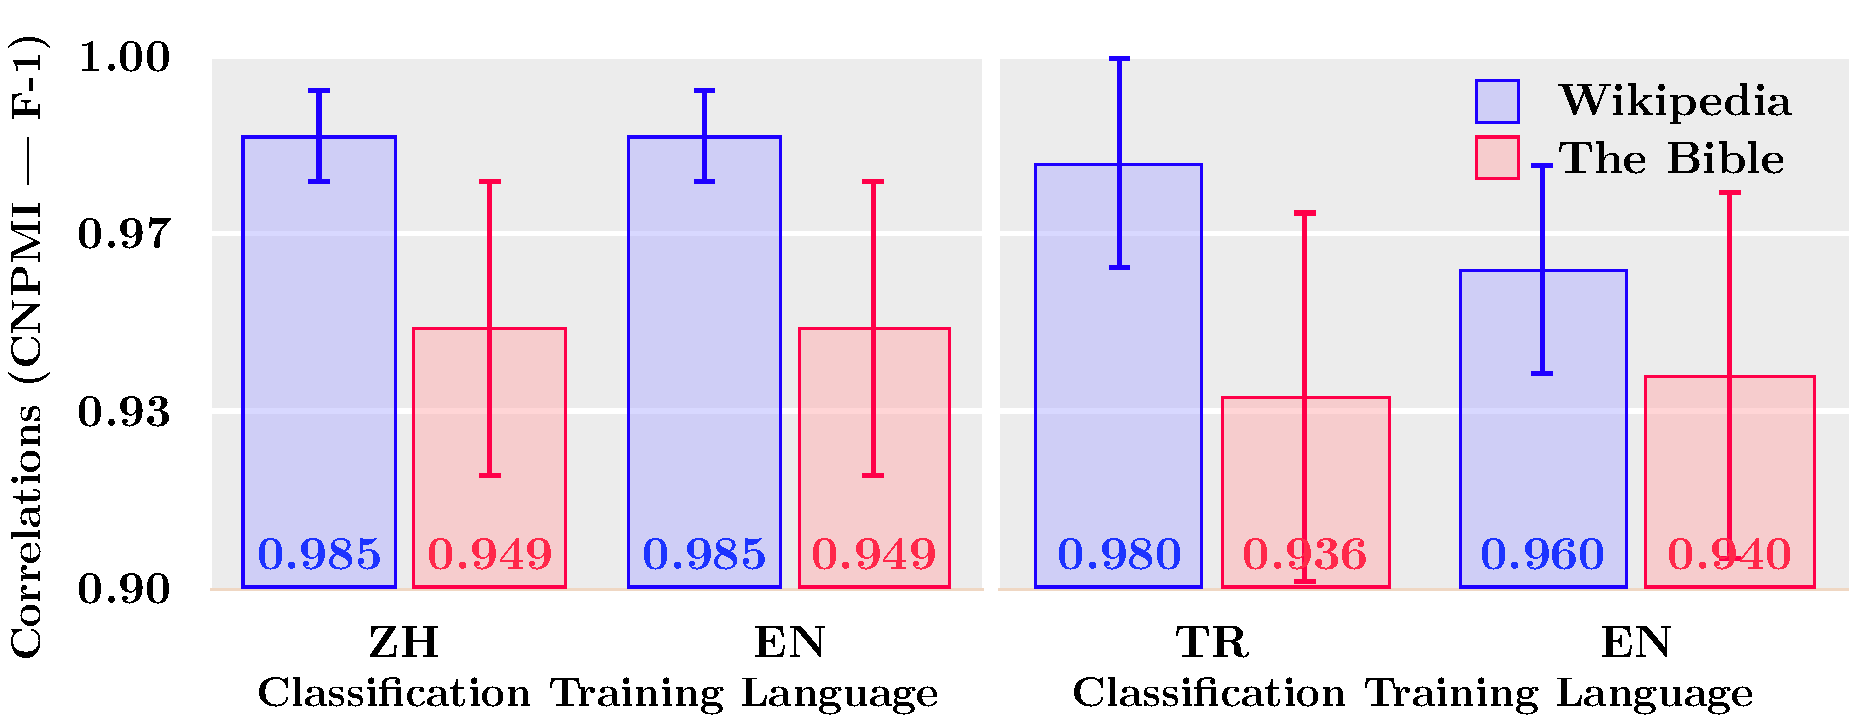
\includegraphics[width=\linewidth]{2018_naacl_mltm_eval/auto_fig/mlc}
	\caption{Pearson correlation between classification F1 scores
		and \cnpmi{}: both \cnpmi{} data sources predict whether a
		classifier using topic features will work well, but
		Wikipedia has slightly higher correlation with lower variance.}
	\label{fig:mlc}
\end{figure}



\subsection{Re-Estimating Model-Level Coherence}

In Section~\ref{sec:estimator}, we improve Bible-based \cnpmi{} scores
for individual topics.  Here, we show the estimator also improves
model-level coherence.  We apply the estimator on the models created
in Section~\ref{sec:add-links} and calculate the correlation between
estimated scores and Wikipedia's \cnpmi{} (Table~\ref{tab:est-model}).

The coherence estimator substantially improves scores except for
Turkish: the correlation is better \emph{before} applying the
estimator ($0.911$). We suspect a lack of overlap between topics
between Turkish and languages other than Chinese is to blame
(Figure~\ref{fig:overlap}); the features used by the estimator do not
generalize well to other kinds of features; training on many languages
pairs would hopefully solve this issue.  Turkish is also
morphologically rich, and our preprocessing completely ignores
morphology.



\begin{figure}[t!]
  \centering
  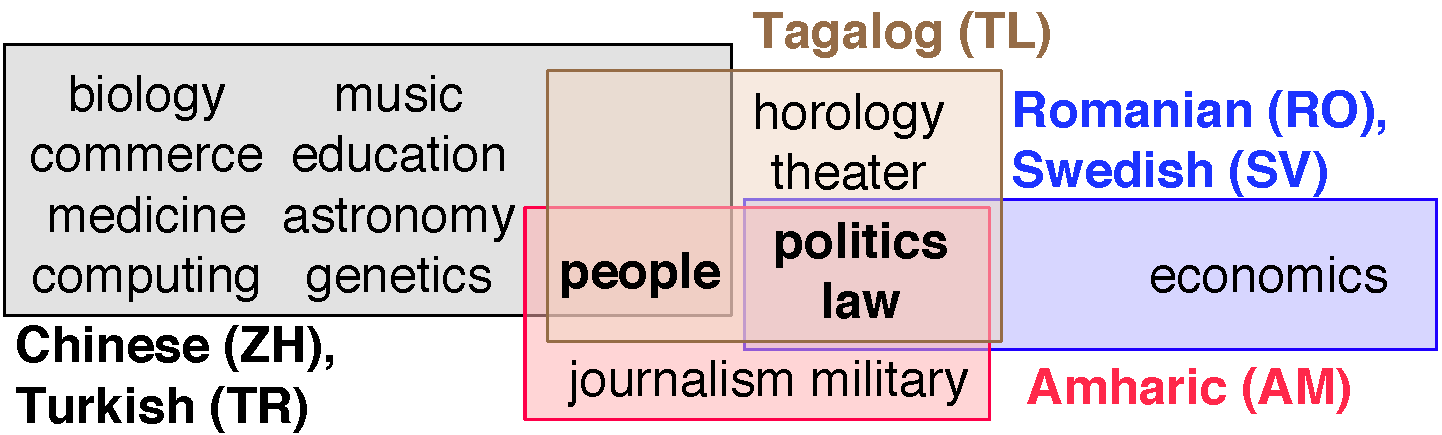
\includegraphics[width=\linewidth]{2018_naacl_mltm_eval/figures/overlap}
  \caption{The overlap of topics and domain: only one out of nine
    Turkish and Chinese topics have domain overlap with Tagalog and
    Amharic topics.  This hinders the Turkish estimator from capturing
    model-level properties.}
	\label{fig:overlap}
\end{figure}


\subsection{Reference Size}
\label{sec:add-ref}


One challenge with low-resource languages is that even if Wikipedia is available,
it may have too few documents to accurately calculate coherence.
As a final analysis, we examine how the reliability of \cnpmi{} degrades
with a smaller reference corpus.


We randomly sample
$20\%$ to $100\%$ of document pairs from the reference
corpora and evaluate the polylingual topic model with all document links
(Figure~\ref{fig:add-ref}), again fixing the cardinality as $10$.

\cnpmi{} is stable across different amounts of reference documents,
as long as the number of reference documents is sufficiently large.
If there are too few reference documents (for example, $20\%$ of Amharic Wikipedia is only $316$ documents),
then \cnpmi{} degrades.






































\begin{figure}[t!]
	\centering
	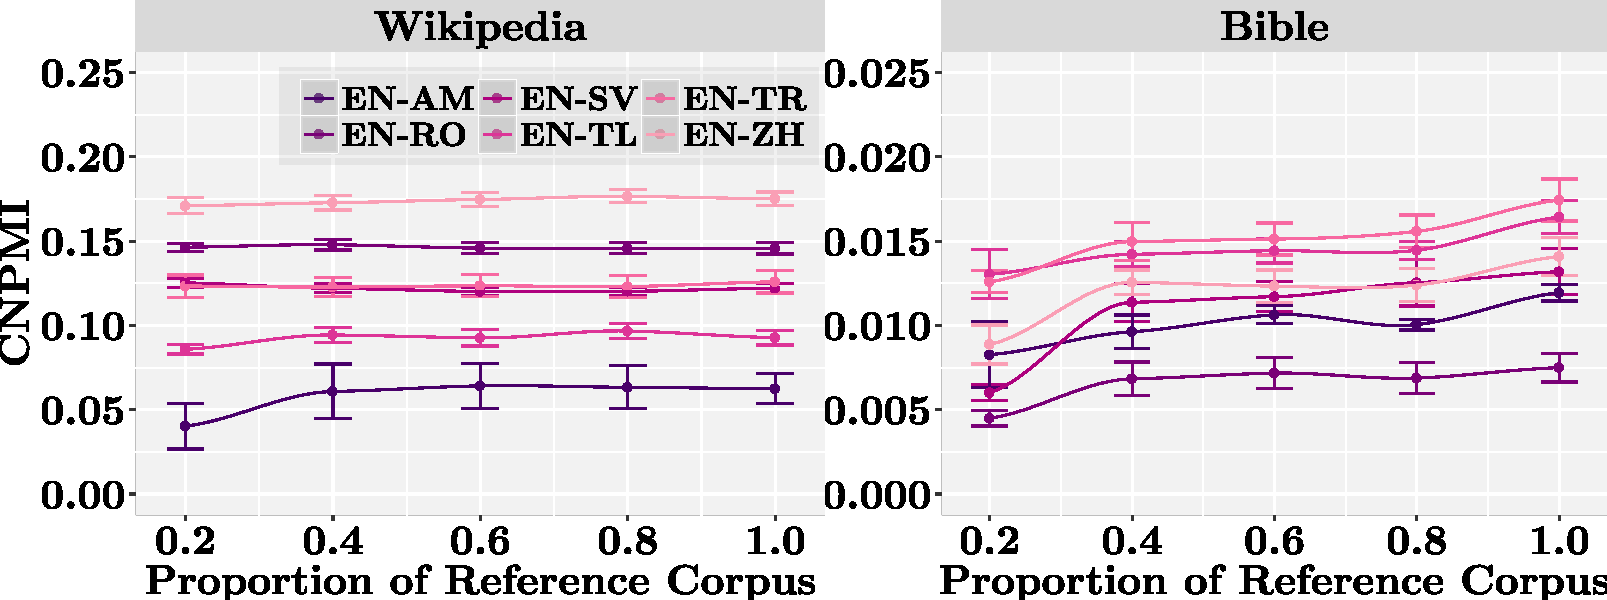
\includegraphics[width=\linewidth]{2018_naacl_mltm_eval/auto_fig/add_ref}
	\caption{\cnpmi{} is stable once the number of reference
          documents is large enough (around five thousand documents).}
	\label{fig:add-ref}
\end{figure}